\documentclass[a4paper, 12pt, oneside]{scrartcl}
%\documentclass[a4paper, 12pt, oneside]{ncc}
\usepackage[warn]{mathtext}          % русские буквы в формулах, с предупреждением
\usepackage[T2A]{fontenc}            % внутренняя кодировка  TeX
\usepackage[utf8]{inputenc}         % кодовая страница документа
\usepackage[english, russian]{babel} % локализация и переносы
\usepackage{indentfirst}   % русский стиль: отступ первого абзаца раздела
\usepackage{misccorr}      % точка в номерах заголовков
\usepackage{cmap}          % русский поиск в pdf
\usepackage{graphicx}      % Работа с графикой \includegraphics{
\usepackage{psfrag}        % Замена тагов на eps картинкаx
\usepackage{caption2}      % Работа с подписями для фигур, таблиц и пр.
\usepackage{soul}          % Разряженный текст \so{ и подчеркивание \ul{
\usepackage{soulutf8}      % Поддержка UTF8 в soul
\usepackage{fancyhdr}      % Для работы с колонтитулами
\usepackage{multirow}      % Аналог multicolumn для строк
\usepackage{ltxtable}      % Микс tabularx и longtable
\usepackage{paralist}      % Списки с отступом только в первой строчке
%\usepackage{longtable}
%\usepackage{tabularx}
\usepackage[perpage]{footmisc} % Нумерация сносок на каждой странице с 1
\usepackage{amsmath}
\usepackage{amsfonts}
\usepackage{amssymb}
\usepackage{tabularx}  %продвинутые таблицы
\usepackage{fancyhdr} %колонтитулы
\usepackage{longtable}
\usepackage[table]{xcolor} %цвета ячеек
% Задаем отступы: слева 30 мм, справа 10 мм, сверху до колонтитула 10 мм
% снизу 25 мм
%\usepackage[a4paper, top=10mm, left=30mm, right=10mm, bottom=25mm]{geometry}
% Нумерация формул, картинок и таблиц по секциям
\numberwithin{equation}{section}
\numberwithin{table}{section}
\numberwithin{figure}{section}
% % % % % % % % % % % % % % % % % % % % % % % % % % % % % % % % % % % % % % % %
% % % % %
\begin{document}
\section{Пункт -1}
В данном отчете все скрипты написаны с использованием языка python3.6 и следующих фрэймфорков, упрощающих рутину: numpy, 
scikit-learn, pandas, seaborn, os, matplotlib. Работа со всеми случайностями в перемешивании, разбиении и инициализации 
возлагается на scikit-learn и его встроенные опции для контроля случайных чисел, такие как random state.

\section{Пункт 0}
Сначала нарисуем попарные диаграммы рассеивания с гистограммами на диагонали. Рисунок слишком большой, чтобы вставлять его в отчет, потому
см. вложенный в архив файл sm.png. Рассмотрим сначала диаграммы рассеяния предикторов и целевой переменной: налицо достаточно сильные 
положительные корреляции целевой переменной и признаков Beds, Baths, Square feet. Ожидаем, что эти признаки внесут в объясненную 
вариацию целевой переменной значительную часть и войдут в уравнение регрессии с положительными коэффициентами. Кроме того, 
заметим, что имеется также чуть менее выраженная отрицательная корреляция целевой переменной с ковариатами Miles to resort, Miles to base.
Далее следует практически полное отсутствие корреляции зависимой переменной с регрессором Acres, слабая положительная корреляция с Cars и
предположительно нелинейная связь с Years old, возможно данная зависимость является квадратичной. Теперь рассмотрим связь предикторов между 
собой: видим, что Beds достаточно сильно положительно коррелирует с Baths и Square feet, следовательно среди регрессоров наблюдается 
явление мультиколлинеарности, которое может скрыть истинные зависимости, поэтому без регуляризации не обойтись. Далее Square feet 
коррелирует с Baths, Miles to resort с Miles to base. В остальном диаграммы рассеяния выглядят либо случайно, либо прослеживается 
некоторая нелинейная связь, которая не должна влиять на модель. На некоторых диаграммах можно заметить выбросы (особенно это заметно 
на гистограмме Years old, Acres)
(правильнее будет сказать influential observations, наверное), которые могут 
вносить шум в модель. \\
В последнюю очередь заметим, что некоторые гистограммы выглядят асимметрично или имеют тяжелые хвосты, а значит взятие логарифма может 
потенциально улучшить результаты, поскольку регрессия хорошо предсказывает те наблюдения, которые близки к средним. Так же можно попробовать 
добавить $$ Years\_old^2  $$ в модель.

\section{Пункт 1}
Для разбиения выборки псевдослучайным образом на обучающую и тестовую воспользуемся встроенной в scikit-learn рутиной из модуля model selection: 
train test split. Зададим seed и необходимые пропорции. Подробности в скрипте main.py.

\section{Пункт 2}
Очевидно, что параметры lasso регрессии будут быстрее сходиться к нулю с увеличением коэффициента регуляризации, чем параметры ridge регрессии, 
поэтому зададим для lasso регрессии диапазон вариации коэффициента меньше, чем для ridge регрессии: 0-150 и 0-300 соответственно. Стандартизуем 
обучающую и тестовую выборки. Нанесем на график линии mean squared error для оптимального константного прогноза, коим является среднее значение 
целевой переменной. Построим 
для каждого выбранного коэффициента регуляризации модель соответствующей регресии. Ниже изображены графики зависимостей метрики mean squared error 
от коэффициента регуляризации по сравнению с оптимальным константным прогнозом.
\begin{figure}[h]
    \centering
    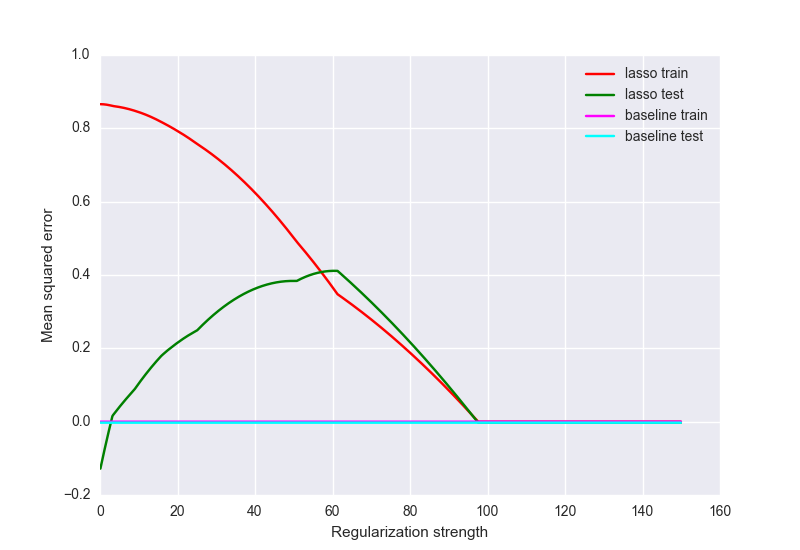
\includegraphics[width=\linewidth]{rss_lasso.png}
\end{figure}
\newline
\begin{figure}[h]
    \centering
    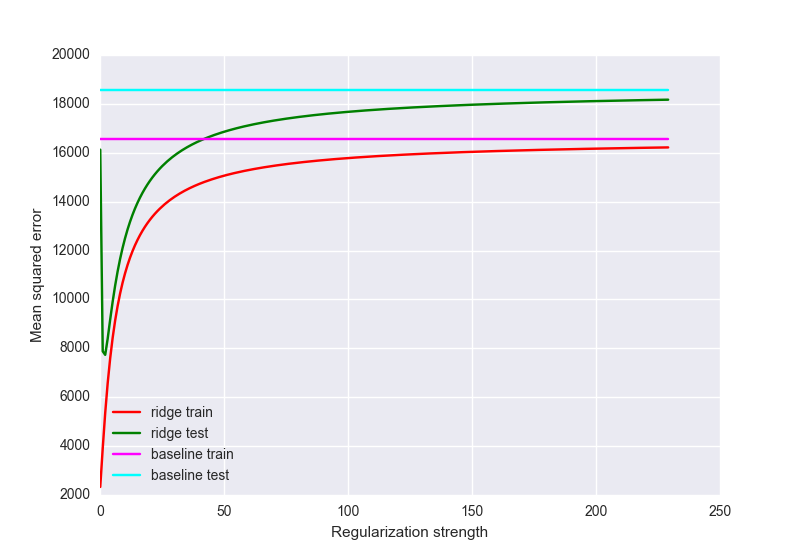
\includegraphics[width=\linewidth]{rss_ridge.png}
\end{figure}

\newpage
Видно, что для обучающих выборок ошибка всюду меньше, чем регрессия на константу, и только при очень сильной регуляризации эта ошибка сходится 
к ошибке константного прогноза, причем для lasso регрессии намного быстрее, чем для ridge регрессии. С другой стороны, на тестовых данных модель сначала 
показывает себя хуже, чем константная, но с увеличением коэффициента регуляризации начинает показывать хорошие значения, после чего сходится к константному прогнозу.

\section{Пункт 3}
Построим графики зависимости коэффициентом линейной регрессии от коэффициента регуляризации. Ниже представлены графики.
\begin{figure}[H]
    \centering
    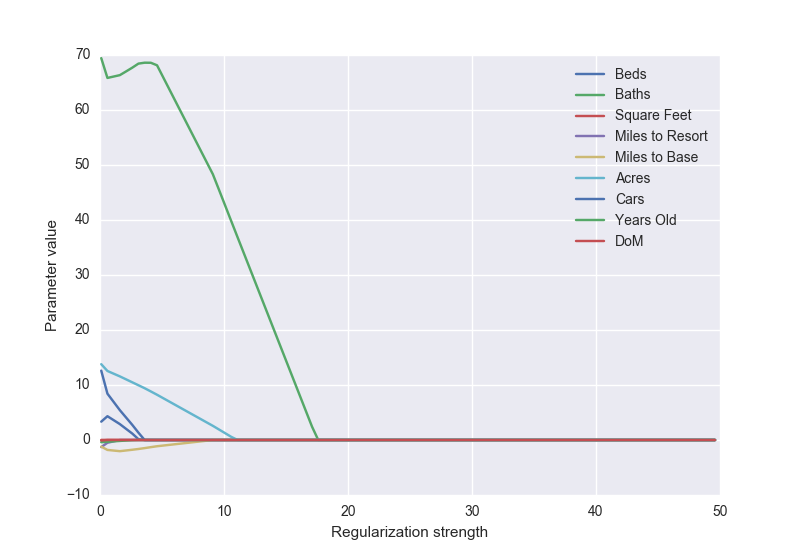
\includegraphics[width=\linewidth]{Lasso_params.png}
\end{figure}

\begin{figure}[H]
    \centering
    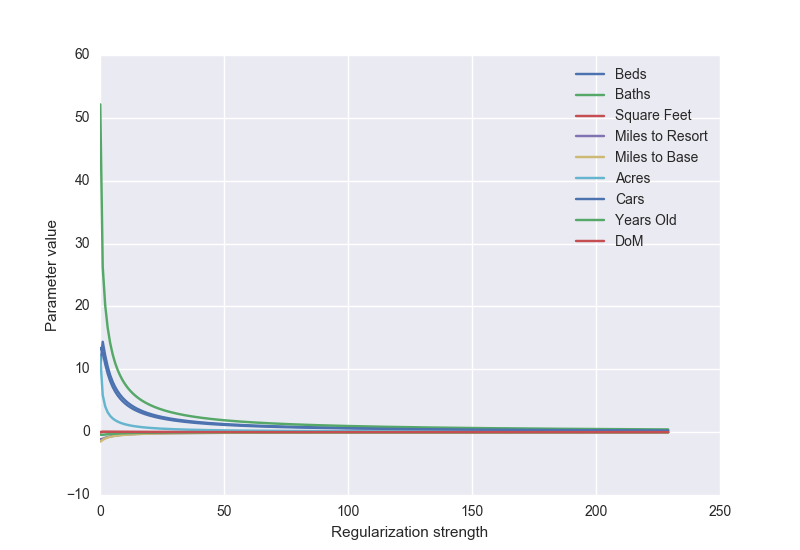
\includegraphics[width=\linewidth]{Ridge_params.png}
\end{figure}

\newpage
\section{Пункт 4}
Согласно графикам выше в лассо регрессии последними в ноль сваливаются признаки Baths, Acres, в ридж регрессии Baths, Square feet. Будем считать их 
наиболее значимыми. Оптимальным методом по результатам теста оказалась модель ridge регрессии с коэффиицентом регуляризации 50.1 со средним квадратом 
отклонения 7601.38, что можно наблюдать на графиках из пункта 3. Значения коэффициентов сохранены в файл results.txt, вложенный в архив с отчетом. 

\section{Пункт 5}
Сначала код напиши

\section{Пункт 6}
Сначала код напиши

\section{Пункт 7}
Сначала код напиши

\end{document}
